\newpage
\section*{Шаблоны с помощью Canva}
\label{sec:templates}

\addcontentsline{toc}{section}{\nameref{sec:templates}}

\subsection*{Шаг 1 (копирование)}
Создайте копию изображения, нажав на вкладку Файл — Сделать копию.
\textbf{Пожалуйста, убедитесь, что вы не вносите изменения в оригинальное изображение.}
\begin{center}
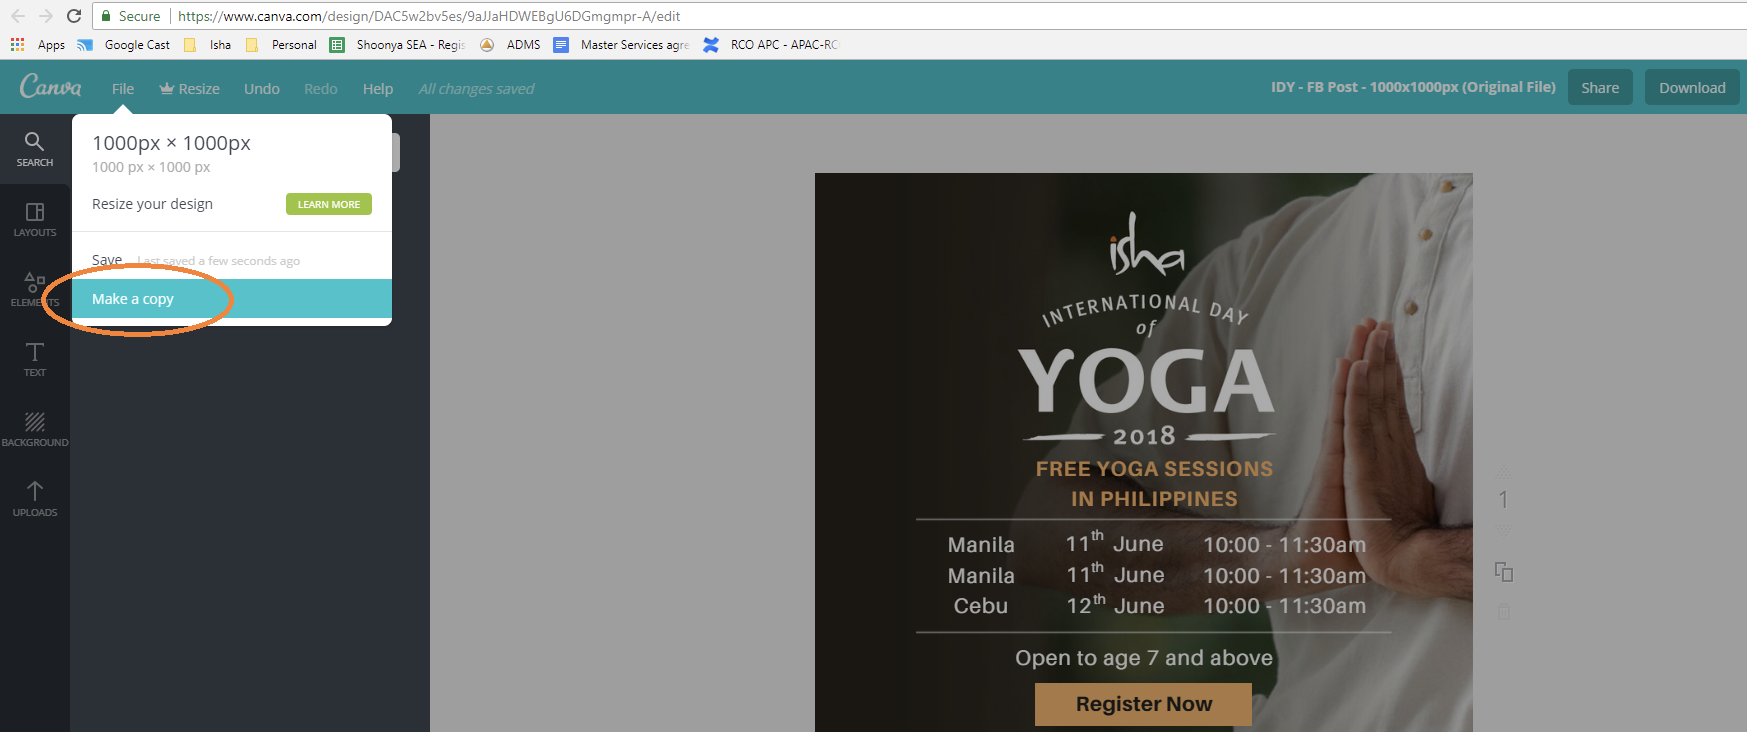
\includegraphics[width=0.99\textwidth]{canva1}
\end{center}

\subsection*{Шаг 2 (изменение)}

Внесите необходимые изменения в тексте изображения. 


\subsection*{Шаг 2a (загрузка, если требуется)}
\begin{enumerate}
\item Загрузите нужное изображение в Canva. 
\item Перетащите нужное изображение в поле для дизайна и внесите необходимые изменения. 
\end{enumerate}

\begin{center}
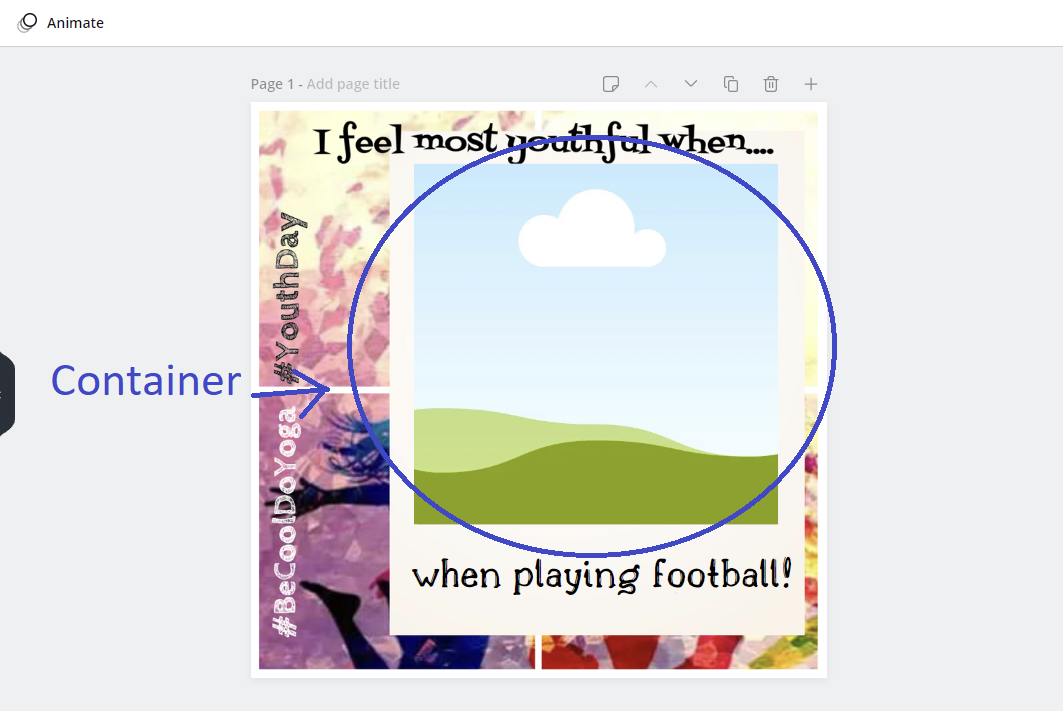
\includegraphics[width=0.59\textwidth]{canva2}
\end{center}


\subsection*{Шаг 3 (экспорт)}
Кликните на кнопку Скачать — Выберите нужный формат изображения: JPEG, PDF и т.д.
\begin{center}
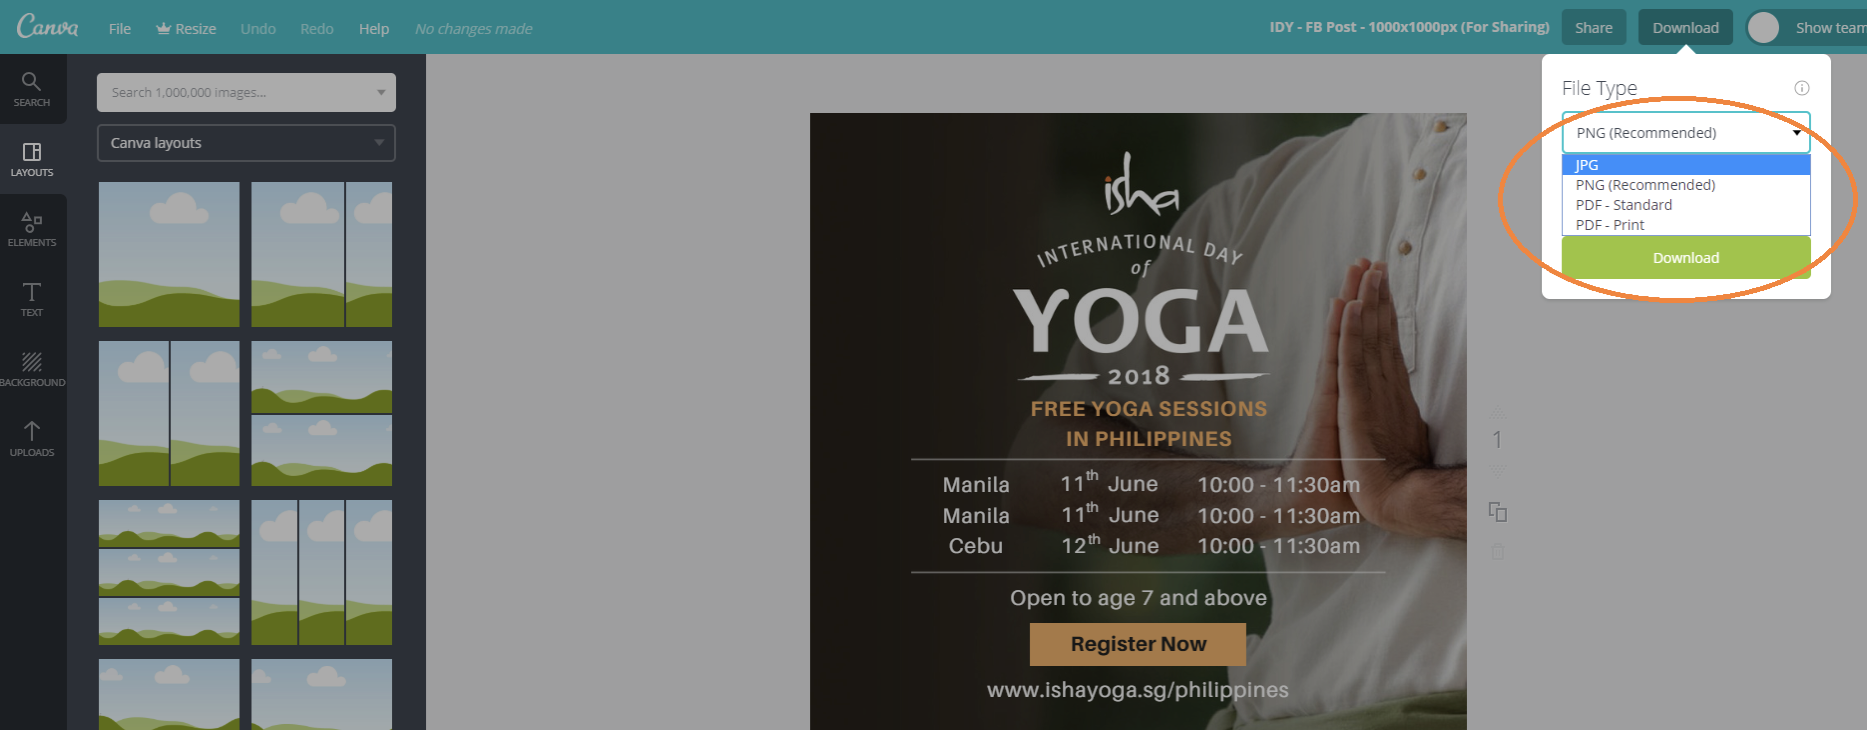
\includegraphics[width=0.99\textwidth]{canva3}
\end{center}


\subsection*{Шаг 4 (радостное использование)}
Откройте скачанное изображение и используйте его для продвижения своих сессий.

